\documentclass{../source/zjureport}

\major{信息工程}
\name{箫宇 }
\title{实验设计报告}
\stuid{ }
\college{信息与电子工程学院}
\date{\today}
\lab{教4-421}
\course{数字信号处理}
\instructor{徐元欣}
\grades{}
\expname{基4-FFT算法编程}
\exptype{验证}
\partner{--}

\begin{document}
    \makeheader

    \section{实验目的和要求}
    FFT是快速计算DFT的一类算法的总称。
    通过序列分解,用短序列的DFT代替长序列的DFT,使得计算量大大下降。基4-FFT是混合基FFT的一个特例。

    通过编写基4-FFT算法程序,加深对FFT思路、算法结构的理解。

    \section{实验内容和步骤}
    编写16点基4-FFT算法的MATLAB程序(studentname.m文件)。

    产生16点输入序列x,用自己的学号作为前10点的抽样值,后面补
    6个零值抽样。算出16点频谱序列X,用stem(X)显示频谱图形。

    \section{主要仪器设备}
    用MATLAB。

    \section{操作方法和实验步骤}
    (参见“二、实验内容和步骤”)

    \section{实验数据记录和处理}
        \subsection{基4-FFT算法思路、流图结构简述如下}
            \subsubsection{算法思路}
            令序列$x(n)$的N点DFT的结果为$X(k)$,且有$N = 4^m$,现按$((n))_4$的结果对序列进行分组,得

            $$\begin{aligned}&x^{(0)}(n)=x(4 n) \\&x^{(1)}(n)=x(4 n+1) \\&x^{(2)}(n)=x(4 n+2) \\&x^{(3)}(n)=x(4 n+3)\end{aligned} \quad 0 \leqslant n \leqslant \frac{N}{4}-1$$
            因而有:
            $$\begin{aligned} X(k)=& \sum_{l=0}^{4^{m-1}-1} x(4 l) W_{N}^{4 k}+\sum_{l=0}^{4^{m-1}-1} x(4 l+1) W_{N}^{(4+1) k}+\sum_{l=0}^{4^{m-1}-1} x(4 l+2) W_{N}^{(4 l+2) k} \\ &+\sum_{l=0}^{4^{m-1}-1} x(4 l+3) W_{N}^{(4 l+3) k}=\sum_{l=0}^{4^{m-1}-1} x^{(0)}(l) W_{4^{m-1}}^{k k-1}+W_{N}^{k} \sum_{l=0}^{4^{m-1}} x^{(1)}(l) W_{4^{m-1}}^{k-1} \\ &+W_{N}^{2 k^{m-1}} \sum_{l=0}^{4-1} x^{(2)}(l) W_{4^{m-1}}^{k}+W_{N}^{3 k^{m-1}} \sum_{l=0}^{4-1} x^{(3)}(l) W_{4^{m-1}}^{k_{k}}=X^{(0)}((k))_{4^{m-1}} \\ &+W_{N}^{k} X^{(1)}((k))_{4^{m-1}}+W_{N}^{2 k} X^{(2)}((k))_{4^{m-1}}+W_{N}^{3 k} X^{(3)}((k))_{4^{m-1}} \\ & 0 \leqslant k \leqslant N-1=4^{m}-1 \end{aligned}$$
            其中:
            $$
                \begin{aligned}
                &X^{(0)}(k)=\operatorname{DFT}_{4^{m-1}}\left\{x^{(0)}(n)\right\} \\
                &X^{(1)}(k)=\operatorname{DFT}_{4^{m-1}}\left\{x^{(1)}(n)\right\} \\
                &X^{(2)}(k)=\operatorname{DFT}_{4^{m-1}}\left\{x^{(2)}(n)\right\} \\
                &X^{(3)}(k)=\operatorname{DFT}_{4^{m-1}}\left\{x^{(3)}(n)\right\}
                \end{aligned}
            $$
            若令$0<=k<=4^{m-1}-1$,则上式可以写作:
            $$
                \left\{\begin{array}{l}
                X(k)=X^{(0)}(k)+W_{N}^{k} X^{(1)}(k)+W_{N}^{2 k} X^{(2)}(k)+W_{N}^{3 k} X^{(3)}(k) \\
                X\left(k+4^{m-1}\right)=X^{(0)}(k)-\mathrm{j} W_{N}^{k} X^{(1)}(k)-W_{N}^{2 k} X^{(2)}(k)+\mathrm{j} W_{N}^{3 k} X^{(3)}(k) \\
                X\left(k+2 \times 4^{m-1}\right)=X^{(0)}(k)-W_{N}^{k} X^{(1)}(k)+W_{N}^{2} X^{(2)}(k)-W_{N}^{3 k} X^{(3)}(k) \\
                X\left(k+3 \times 4^{m-1}\right)=X^{(0)}(k)+\mathrm{j} W_{N}^{k} X^{(1)}(k)-W_{N}^{2 k} X^{(2)}(k)-\mathrm{j} W_{N}^{3 k} X^{(3)}(k)
                \end{array}\right.
            $$

            \subsubsection{流图结构}
            \begin{figure}[H]
                \centering
                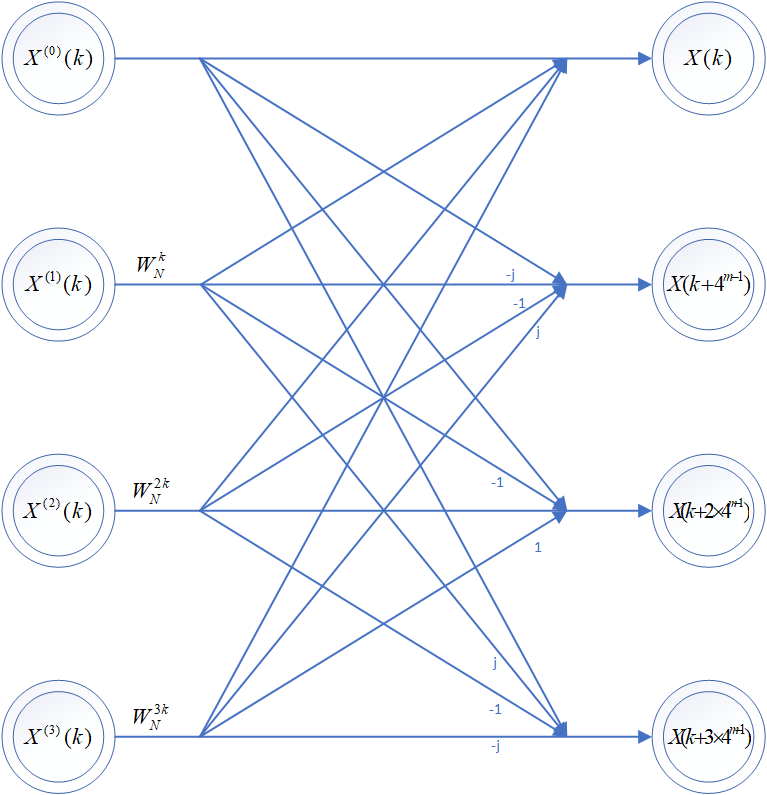
\includegraphics[scale = 0.5]{figure/基础蝶形运算.png}
                \caption{流图结构}
            \end{figure}

        \subsection{16点基4-FFT算法的流图绘出如下}
        \begin{figure}[H]
            \centering
            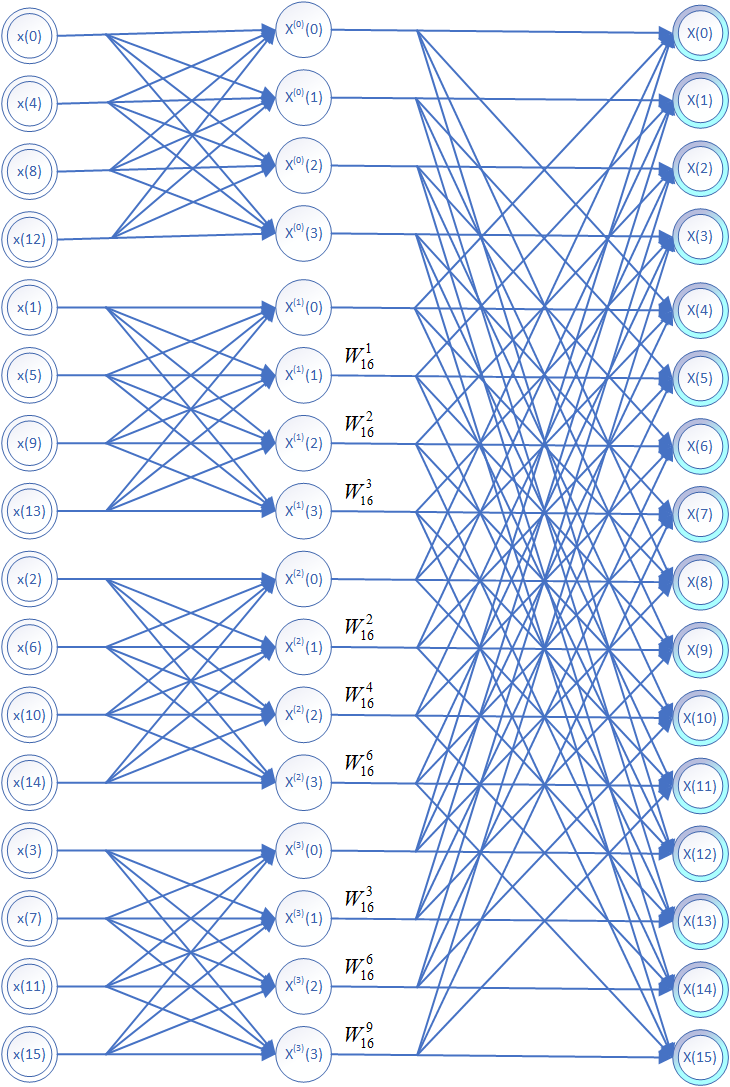
\includegraphics[scale = 0.7]{figure/流图.png}
            \caption{16点基4-FFT算法的流图}
        \end{figure}

        \subsection{16点基4-FFT算法的MATLAB程序(studentname.m)列出如下}
        \lstinputlisting[caption = 绘图函数 , language = matlab]{code/studentname.m}

        \subsection{用自己的学号构成的输入序列为(列出数值,插入图形)}
            \subsubsection{数值}
            x = [3 1 9 0 1 0 5 0 5 5 0 0 0 0 0 0]
            \subsubsection{图形}
            \begin{figure}[H]
                \centering
                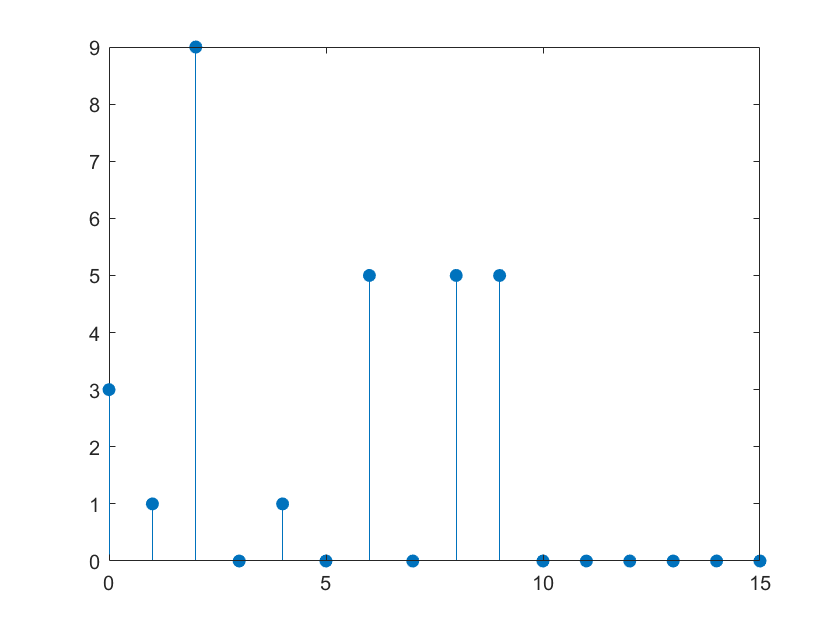
\includegraphics[scale = 0.5]{figure/学号.png}
                \caption{学号}
            \end{figure}

        \subsection{对应的输出频谱序列为(列出数值,插入图形)}
            \subsubsection{数值}
                \begin{table*}[]
                    \begin{tabular}{|l|l|l|l|l|l|l|l|}
                    \hline
                    \multicolumn{1}{|c|}{\textbf{1}}       & \multicolumn{1}{c|}{\textbf{2}}        & \multicolumn{1}{c|}{\textbf{3}}       & \multicolumn{1}{c|}{\textbf{4}}         & \multicolumn{1}{c|}{5}                 & \multicolumn{1}{c|}{6}                 & \multicolumn{1}{c|}{7}                 & 8                                      \\ \hline
                    17.0000+0.0000i                        & {\color[HTML]{000000} 4.5239-12.4302i} & {\color[HTML]{000000} 2.7574+0.2426i} & {\color[HTML]{000000} -3.2977-12.5950i} & {\color[HTML]{000000} -5.0000+6.0000i} & {\color[HTML]{000000} -6.3592+5.2040i} & {\color[HTML]{000000} 11.2426+8.2426i} & {\color[HTML]{000000} -2.8671+9.3688i} \\ \hline
                    \multicolumn{1}{|c|}{9}                & \multicolumn{1}{c|}{10}                & \multicolumn{1}{c|}{11}               & \multicolumn{1}{c|}{12}                 & \multicolumn{1}{c|}{13}                & \multicolumn{1}{c|}{14}                & \multicolumn{1}{c|}{15}                & 16                                     \\ \hline
                    {\color[HTML]{000000} 17.0000+0.0000i} & {\color[HTML]{000000} 4.5239-12.4302i} & {\color[HTML]{000000} 2.7574+0.2426i} & {\color[HTML]{000000} -3.2977-12.5950i} & {\color[HTML]{000000} -5.0000+6.0000i} & {\color[HTML]{000000} -6.3592+5.2040i} & {\color[HTML]{000000} 11.2426+8.2426i} & {\color[HTML]{000000} -2.8671+9.3688i} \\ \hline
                    \end{tabular}
                    \end{table*}

            \subsubsection{图形}
            \begin{figure}[H]
                \centering
                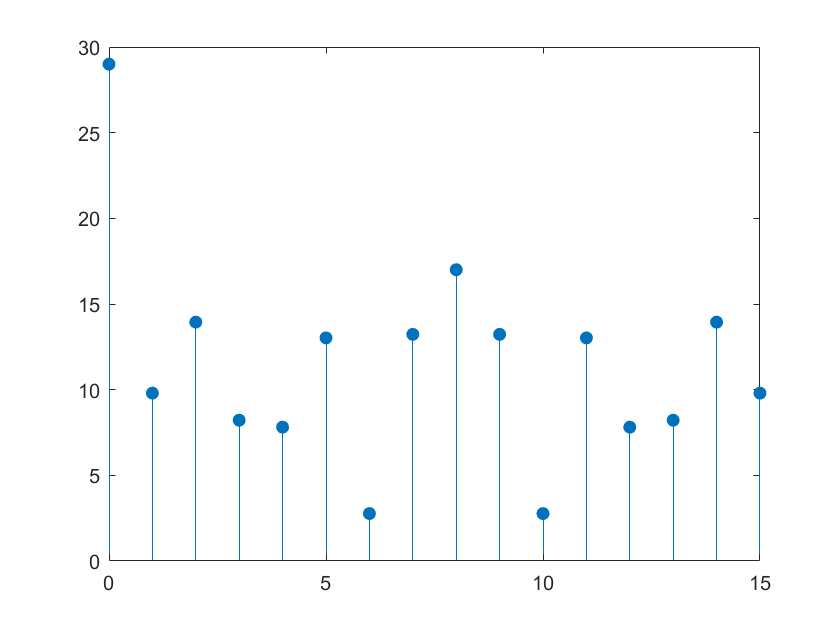
\includegraphics[scale = 0.5]{figure/频谱.png}
                \caption{频谱}
            \end{figure}
    \section{实验结果与分析}
        与系统自带得fft函数结果进行比较后,可以看出结果具有正确性。

        同时,同基2时域抽选法相比,基4所需的复乘次数降低,而复加次数则有所上升,因为复乘有着较大
        的运算开销,因此复乘次数的减少有利于改进FFT的计算效率

\end{document}
